\documentclass{article}

\usepackage{caption}
\usepackage{graphicx}
\usepackage{float}
\usepackage{enumitem}
\usepackage{hyperref}
\usepackage{units}
\usepackage{mhchem}

\begin{document}
	\tableofcontents
	
	\section{Cell cycle}
	
	\begin{figure}[H]
		\centering
		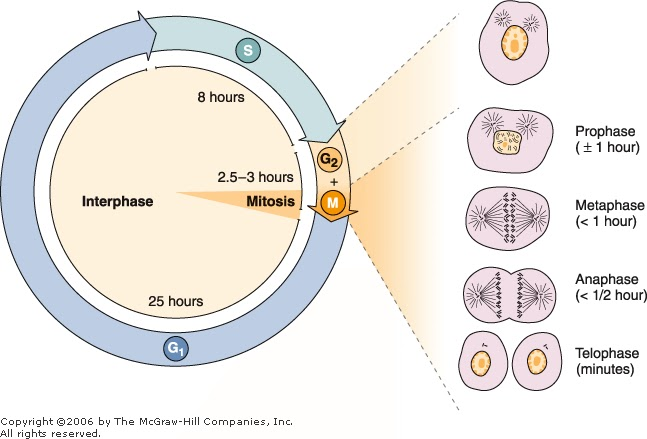
\includegraphics[width=0.8\linewidth]{durations.jpg}
		\caption{\url{https://dehistology.blogspot.com/2011/06/cell-cycle.html}}
	\end{figure}
	
	\subsection{Cdks}
	Cyclin-Dependent Kinases (CDKs) phosphorylate proteins that drive the cell through the cell cycle. This is regulated by
	
	\begin{enumerate}
		\item Synthesis rate of the Cyclins
		\item Ubiquitylation rate of the cyclins (marking them for proteolysis/degradation)
		\item Phosphorylation of the Cdks
		\item CKIs
	\end{enumerate}
	
	\subsection{Cyclins}
	Cyclins activate the CDKs (partially) by forming complexes (see table). There are 4 types of cyclins (A, B, D and E) with various related forms (i. e. D1, D2 and D3 in humans). When characterized by the state of the cell cycle they are active in, they can further be divided into 4 groups: G1/S-Cyclins, S-Cyclins, M-Cyclins and G1-Cyclins.
	
	\begin{table}[h]
		\centering
		\begin{tabular}{|c|c|c|} \hline
			Cyclin & Cdks & Complex \\ \hline
			Cyclin-D & (Cdk4/Cdk6)  & G1-Cdk \\ \hline
			Cyclin-E & Cdk2         & G1/S-Cdk \\ \hline
			Cyclin-A & (Cdk2/Cdk1)  & S-Cdk (MPF) \\ \hline
			Cyclin-B & Cdk1         & M-Cdk (MPF)\\ \hline
		\end{tabular}
		\caption{Cyclines and the Cdks they form complexes with}
	\end{table}

	\begin{enumerate}[label=\textbullet]
		\item G1-Cdk triggers the cell cycle (point of no return)
		\item G1/S-Cdk initiates the cell cycle in the dormant G1 phase  (yeast: START, mammals: restriction point)
		\item S-Cdk triggers transition from the G1 to the S phase 
		\item M-Cdk triggers transition from the G2 to the M phase 
	\end{enumerate}

	The resulting complex when Cyclin A or B bind to Cdk1/Cdk2 is called the maturation promoting factor (MPF).
	
	\begin{figure}[H]
		\centering
		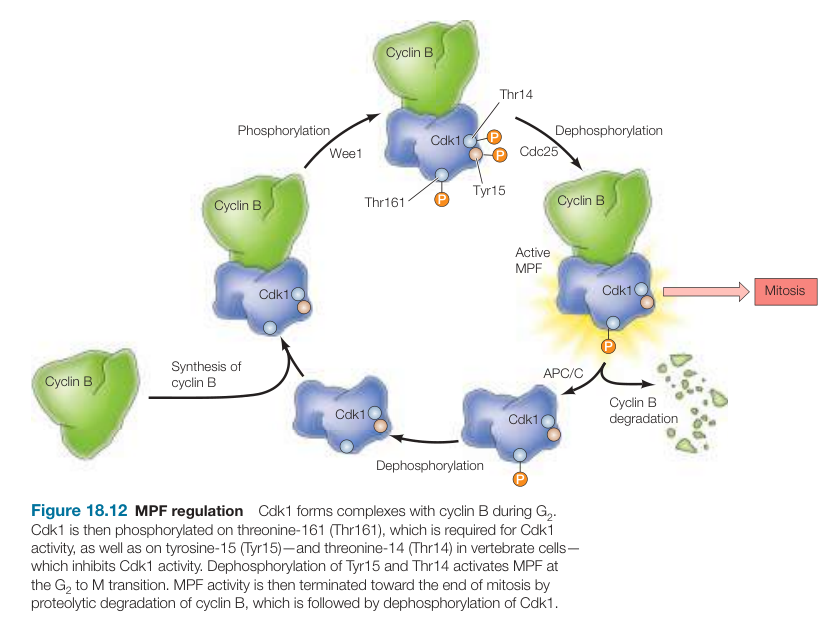
\includegraphics[width=\linewidth]{mpf_regulation_cooper.png}
		\caption{MPF Regulation. The "Phosphorylation" step is carried out by CAK}
	\end{figure}

	Cdk concentration remains mostly constant.\footnote{albert, p. 1093} Concentration of cyclins changes during the cell cycle (see images).
	
	\begin{figure}[H]
		\centering
		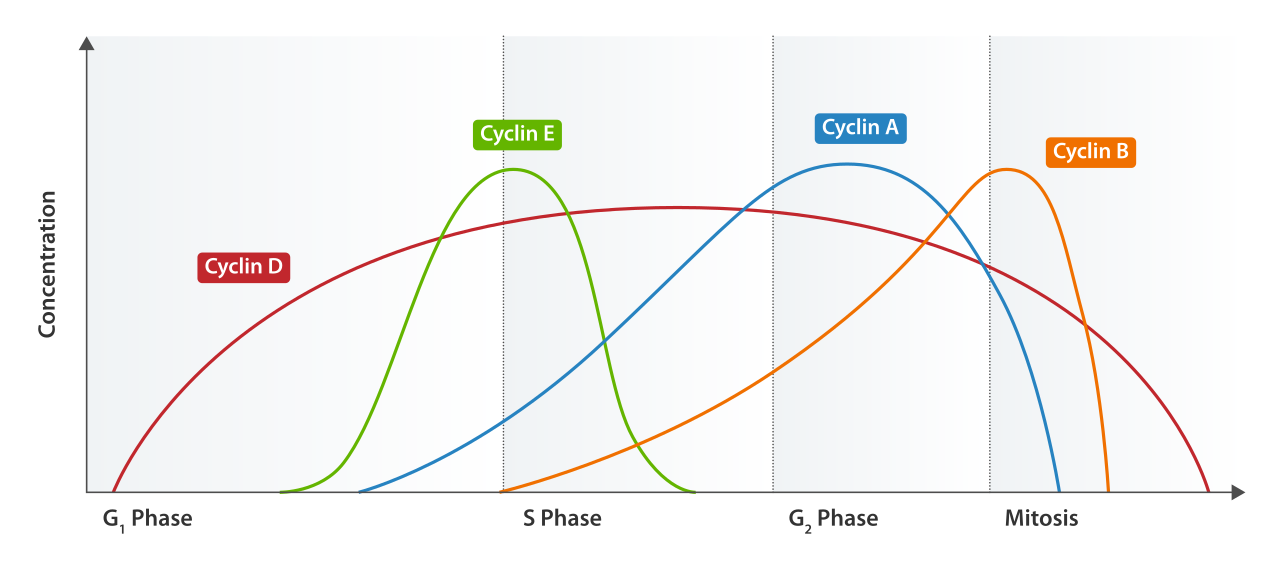
\includegraphics[width=\linewidth]{cyclin_activity_wikipedia.png}
		\caption{Concentration of the cyclins during the cell cycle (wikipedia)}
	\end{figure}
	
	\begin{figure}[H]
		\centering
		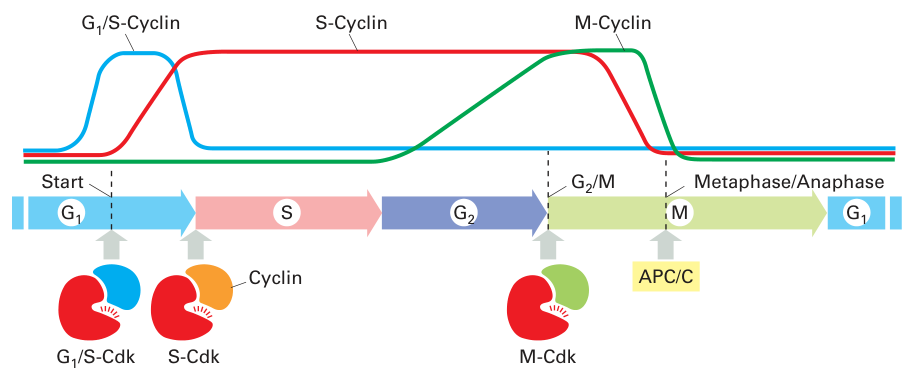
\includegraphics[width=\linewidth]{cyclin_activity_alberts.png}
		\caption{Concentration of the cyclins during the cell cycle (alberts)}
	\end{figure}
	
	\begin{figure}[H]
		\centering
		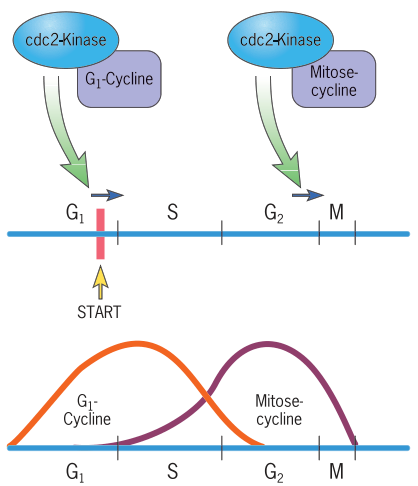
\includegraphics[width=0.8\linewidth]{cyclin_activity_karp.png}
		\caption{Concentration of the cyclins during the cell cycle (karp). cdc2 = cdk1}
	\end{figure}

	\subsubsection{Cyclin A}
	Cyclin A can bind to Cdk2 (replacing Cyclin E), causing the cell to go through with the S phase by initiating DNA replication, and Cdk1, causing transition from the G2 to M phase. Cyclin A/Cdk1 in the late G2 phase activates Cyclin B/Cdk1, which in return causes Cyclin A to be ubiquitylized and eventually degraded. Humans have 2 subforms: Cyclin A1, which is expressed during embryogenesis, and A2, expressed in dividing somatic cells.\footnote{\url{https://en.wikipedia.org/wiki/Cyclin_A}}\\
	
	\subsection{Wee1}
	Wee1 inhibits Cyclin-Cdk complexes by phosphorylation, causing a delay of the M-Phase so that the cell can grow. If Wee1 is defective, the cells transition directly from S- to M-Phase without the growth in the G2 phase, resulting in \textit{wee} little cells :)
	
	\subsection{Cdc25}
	Cdc25 activates the MPF that was previously inactivated by Wee1. It dephosphorylizes Thr14 and Tyr15. Mammals have 3 related forms Cdc25A, B and C.
	
	\subsection{APC/C}
	The anaphase-promoting complex/cyclosome (APC/C) is a ubiquitin ligase and triggers transition from the metaphase to the anaphase by ubiquitylation of securin and Cyclin-A/Cyclin-B, marking them for proteolysis. Once they are destroyed, the MPF is no more.
	
	\subsubsection{Cdc20}
	Binds with APC/C in mitosis to specify target proteins.
	
	\subsubsection{Cdh1}
	Binds with APC/C in late mitosis/G1 to specify target proteins.
	
	\subsection{SCF}
	Skp, Cullin, F-box containing complex is another ubiquitin ligase. SCF ubiquitylates CKIs in the late G1 phase, thus activating S-Cdks; it's also responsible for proteolysis of G1/S-Cdks in the early S phase. Marks p27. Typically requires phosphorylated targets.
	
	\subsubsection{F-Box-Proteins}
	Exchangeable part of the SCF, specifying the target protein. There are more than 70 genes coding for F-Box-Proteins.\footnote{alberts, p. 178}
	
	\subsection{CKIs}
	Cdk inhibitors (CKIs) inhibit Cyclin-Cdk complexes by binding to them (mostly G1/S- and S-Cdks). There are 2 families of CKIs, binding to different Cdks and Cyclin/Cdk complexes:
	
	\begin{figure}[H]
		\centering
		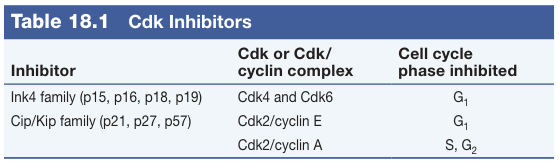
\includegraphics[width=\linewidth]{ckis_cooper.png}
		\caption{CKI families and their targets}
	\end{figure}

	\subsubsection{p27}
	Inhibits Cdks in G1. Gets phosphorylated by Cdk1, causing it to be marked for proteolysis (by SCF or APC/C?). 
	
	\subsubsection{p21}
	Inhibits G1/S-Cdk und S-Cdk if DNA damage occured.
	
	\subsubsection{p16}
	Inhibits G1-Cdk in G1. Frequently inactive in cancer cells.
	
	\subsection{CAK}
	CDK-activating kinase (CAK) activates the cyclin-CDK complex.\footnote{\url{https://en.wikipedia.org/wiki/CDK-activating_kinase}}
	
	\subsection{Rb}
	When dephosphorylated, the retinoblastoma protein (Rb) binds E2F transcription factors, causing them to suppress gene expression that would lead to the cell progressing from G1 to the S-phase. Rb and other pocket proteins are mono-phosphorylated by G1-Cdk and thus inactivated.\footnote{\url{https://en.wikipedia.org/wiki/Retinoblastoma_protein}} During M-to-G1 transition, Rb is dephosphorylated again by PP1. Rb is responsible for keeping cells in G0 and delaying the transition from G1 to S-phase and DNA-replication in case of DNA-damage.
	
	\section{Math stuff}
	
	\subsection{Bimolecular Reaction $A + B \rightarrow C$}
	%TODO: Identify relevant reaction types (A+B->C, A+B->AB, A+B->AC, ...)
	Let's look at 2 proteins A and B participating in the bimolecular reaction \footnote{Chapter mostly copied from Wedler, G.; Freund, H.: Lehr- und Arbeitsbuch Physikalische Chemie. 7. Auflage, S. 565ff.}
	
	\begin{equation}
	\ce{A + B <=>[\ce{k_1}][\ce{k_{-1}}] {AB} ->[\ce{k_2}] C.}
	\end{equation}

	For this we get the speed laws
	
	\begin{align}
		\frac{d[{\ce{AB}}]}{dt} &= \ce{k_1[A][B]} - \ce{k_{-1}[AB]} - \ce{k_2[C]}\\
		\frac{d\ce{[C]}}{dt} &= \ce{k_2[{AB}]}
	\end{align}
	
	Assuming a quasi-static process, we can set $\frac{d[{\ce{AB}}]}{dt} = 0$: The intermediate product is short-lived and its concentation approximately constant. With this, we get
	
	\begin{equation}
		\frac{d\ce{[C]}}{dt} = \frac{k_1k_2}{k_{-1}+k_2}\ce{[A][B]}.
	\end{equation}	
	
	For the intermediate to be short-lived, there are 2 different cases to look at.
	
	\subsubsection{Diffusion-controlled reaction speed}
	Here, we have $k_2 \gg k_1$ and $k_2 \gg k_{-1}$. In that case, we get
	
	\begin{equation}
		\frac{d\ce{[C]}}{dt} = r \approx k_1\ce{[A][B]}.
	\end{equation}
	
	This is the reaction speed $r$ in units $\frac{mol}{s\cdot m^3}$, which is what we want. To calculate how many B molecules collide with A moculecules each second, we can calculate the flow of B through a sphere of radius $r$ around A using Fick's first law. It gives the flow rate of molecules perpendicular to a given area in $\unit[]{\frac{mol}{m^2\cdot s}}$: 
	
	\begin{equation}
		J_N = -D\frac{dN}{dz}
	\end{equation}

	We'll replace $z$ with the radius $r$ (which is perpendicular to the surface), take the absolute value and multiply with the surface of the sphere to get number of molecules per second passing through the surface of the sphere:
	
	\begin{equation}
		J_B = 4\pi r^2D_B\frac{dN_B}{dr}
	\end{equation}

 
	
	\begin{equation}
		k_1 = 4\pi (D_A + D_B)(r_A + r_B)L. 
	\end{equation}

	$D$ is the diffusion coefficient, $r$ the radius of the protein and $L = \unit[2.687\cdot10^{25}]{m^{-3}}$ is the Loschmidt constant. If we use the molecule counts $N_A$ and $N_B$ directly instead of the concentrations, $L$ must be omitted.\\
	$D$ can be calculated using the Stokes-Einstein equation:
	
	\begin{equation}
		D = \frac{k_BT}{6\pi\eta R_0}
	\end{equation}

	where $k_B = \unit[1.381\cdot10^{-23}]{\frac{J}{K}}$ is the Boltzmann constant, $T$ is the temperature, $\eta$ is the viscosity of the fluid and $R_0$ is the hydrodynamic radius of the protein. We will use the approximation $r \approx R_0$. The literature value for the viscosity of the cytoplasma seems to be about $\unit[2]{cP} = \unit[2]{mPa\cdot s}$.\footnote{Luby-Phelps, K.: Cytoarchitecture and Physical Properties of Cytoplasm: Volume, Viscosity, Diffusion, lntracellular Surface Area} We will not use the Arrhenius equation
	
	\begin{equation}
		\eta = A\exp{\left(-\frac{E_a}{RT}\right)}
	\end{equation}

	and simply assume $\eta$ to be constant. Putting it all together, we have
	
	\begin{equation}
		k_1 = \frac{2}{3\eta}k_BTL
	\end{equation}

	\subsubsection{Numbers}
	
	We will use 
	
	\begin{align*}
		k_B &= \unit[1.381\cdot10^{-23}]{\frac{kg\cdot m^2}{K\cdot s^2}}\\
		T &= \unit[310]{K}\\
		L &= \unit[2.687\cdot10^{25}]{m^{-3}}\\
		\eta &= \unit[2\cdot10^{-3}]{\frac{kg}{m\cdot s}}\\
		r_A &= \unit[10\cdot10^{-10}]{m}\\
		r_B &= \unit[40\cdot10^{-10}]{m}\\
		\ce{[A]} &= \unit[1]{\frac{mol}{m^3}}\\
		\ce{[B]} &= \unit[0.1]{\frac{mol}{m^3}}
	\end{align*}
	
	\begin{align}
		\frac{d\ce{[C]}}{dt} &\approx 4\pi(D_A + D_B)(r_A + r_B)L\ce{[A][B]}\\
		&= \frac{4\pi k_BT}{6\pi\eta}\left(\frac{1}{r_A}+\frac{1}{r_B}\right)(r_A+r_B)L\ce{[A][B]}\\
		&= \frac{2k_BTL}{3\eta}\frac{(r_A+r_B)^2}{r_Ar_B}\ce{[A][B]}\\
		&= 
	\end{align}
	
	\subsubsection*{Reaction-controlled reaction speed}
	$k_{-1} \gg k_2$

\end{document}